\documentclass[12pt,a4paper]{article}

% --- Paquetes de Idioma y Formato ---
\usepackage[utf8]{inputenc}
\usepackage[spanish, es-tabla]{babel}
\usepackage[margin=2.5cm]{geometry}
\usepackage{setspace}
\onehalfspacing 
\usepackage{parskip}
\usepackage[hidelinks]{hyperref}

% --- Paquetes de Imágenes ---
\usepackage{graphicx}
\graphicspath{ {./imagenes/} } % Busca en tu carpeta 'imagenes'

% --- Configuración de la Portada ---
\title{
    \vspace{2cm} % Espacio superior
    {\Huge \textbf{Informe Previo TFG: Agentes Autónomos y Sistemas Multi-Agente (MAS)}} \\[1.5cm]
    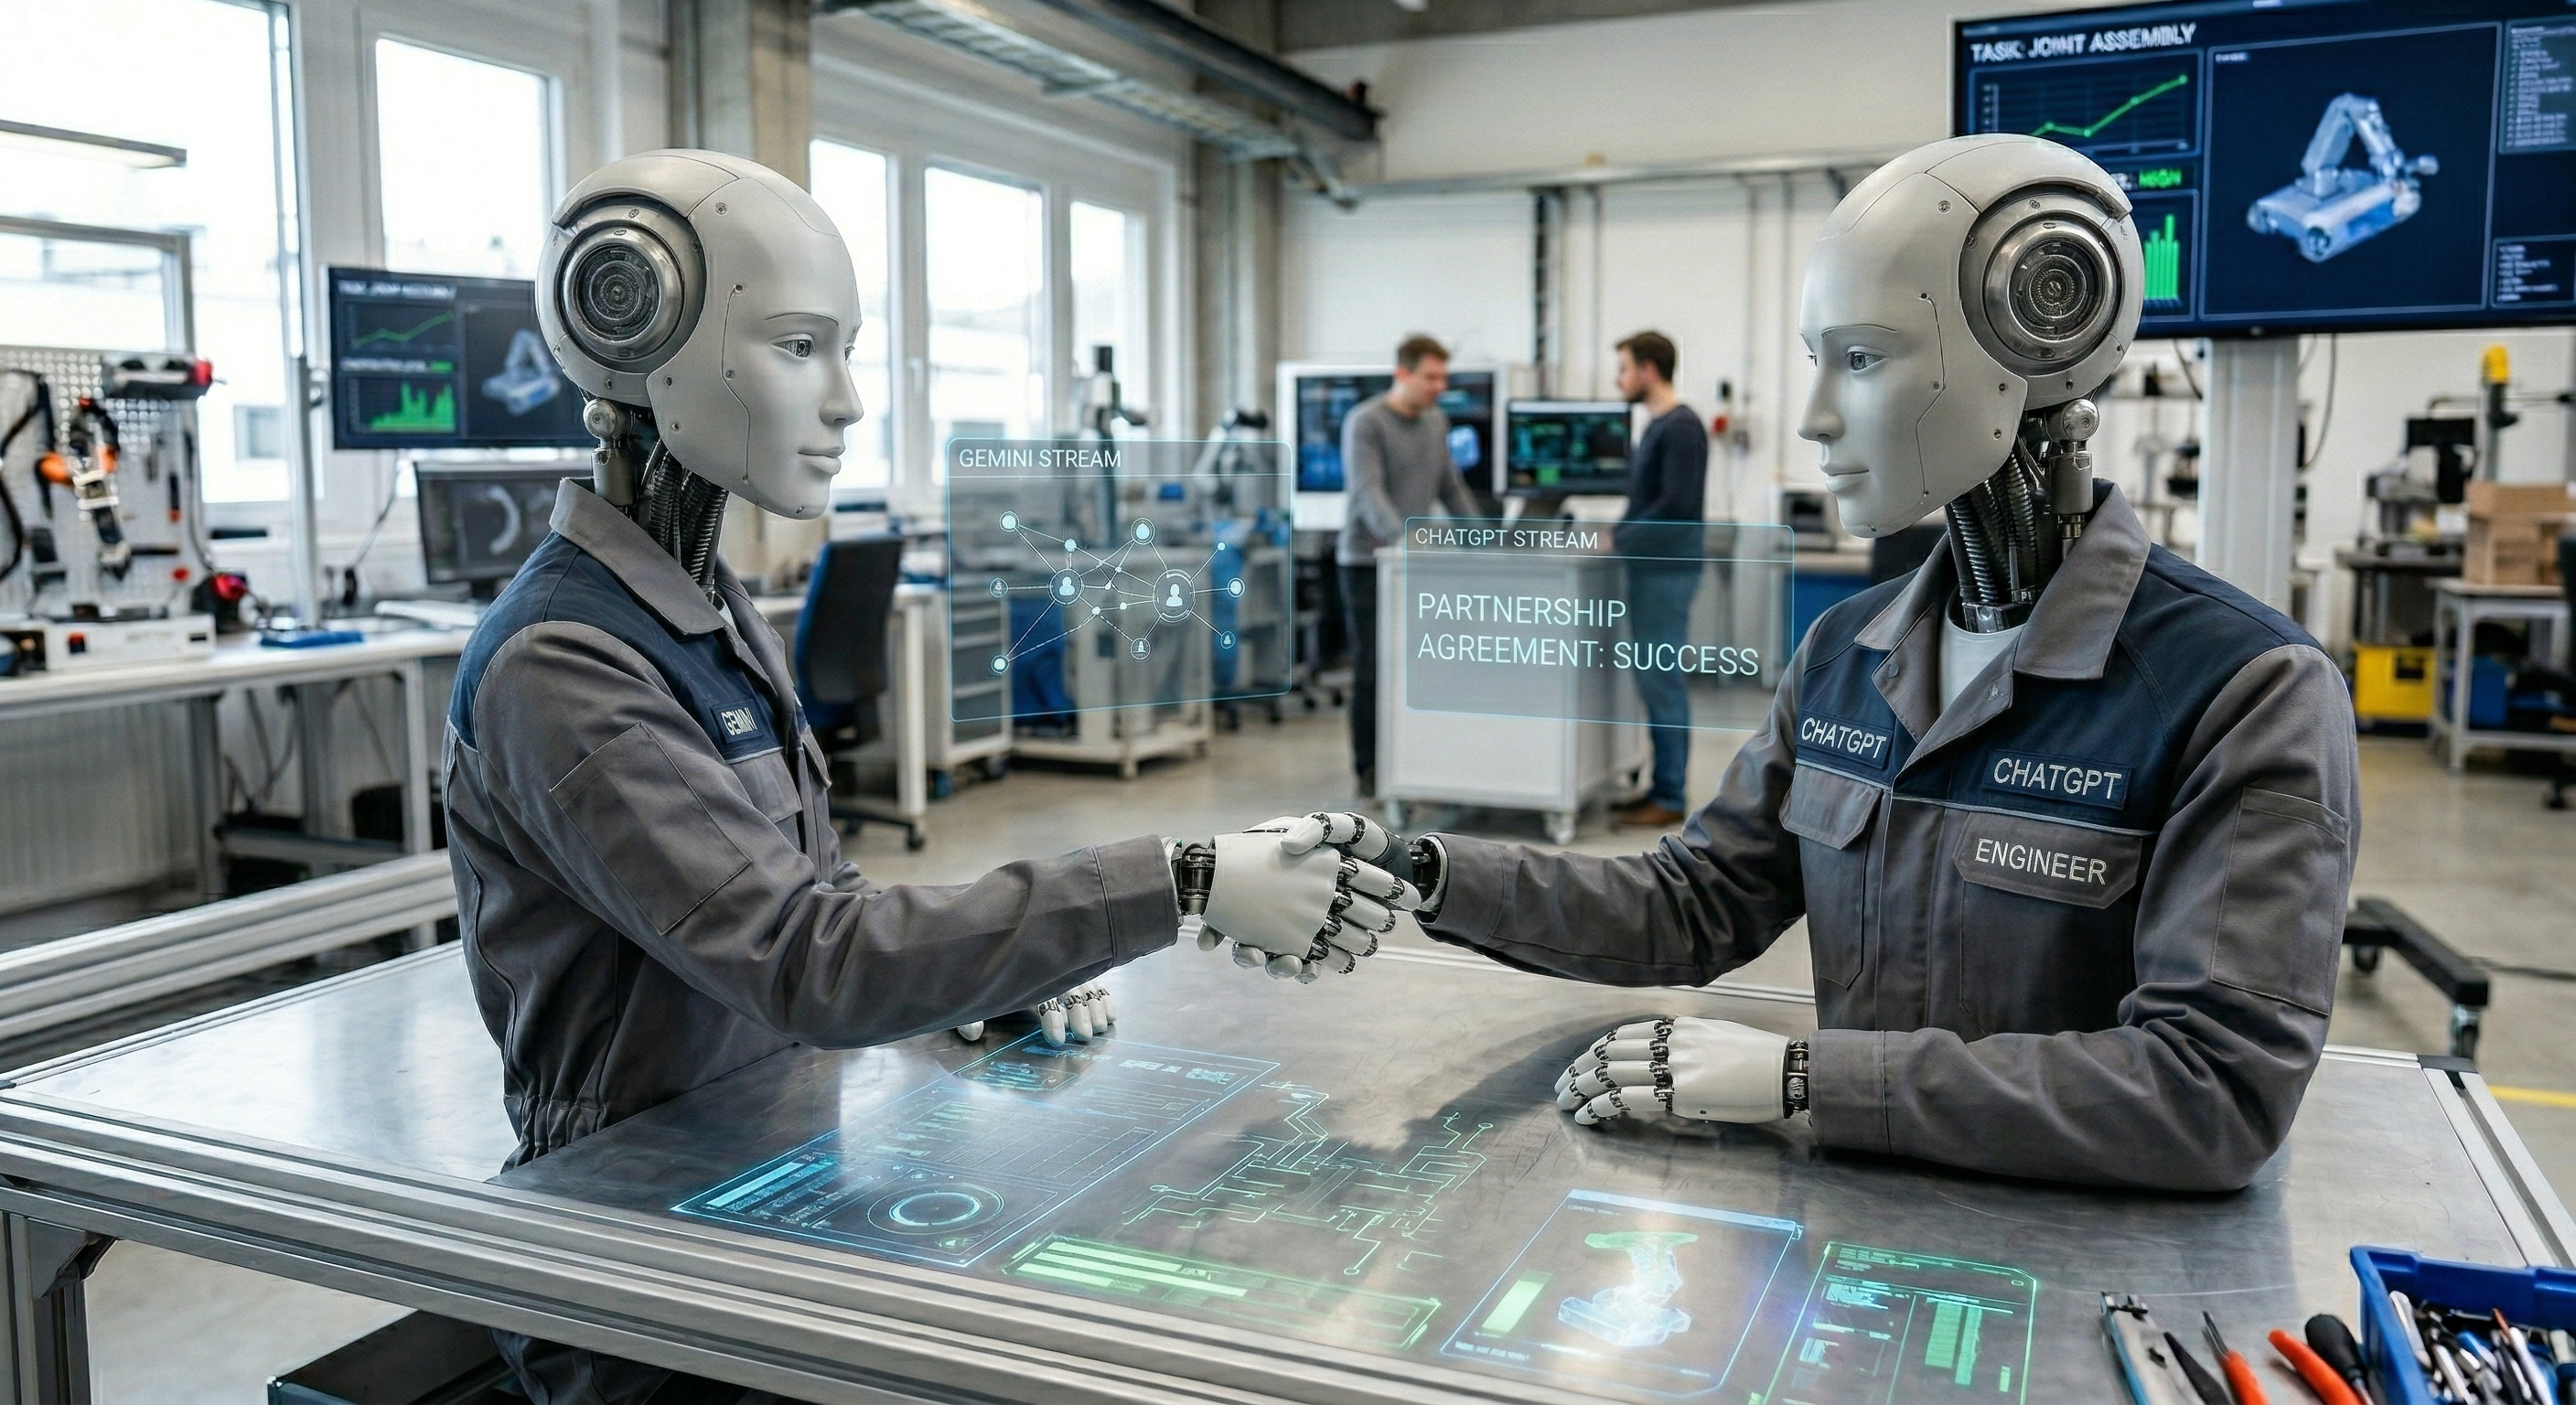
\includegraphics[width=0.5\textwidth]{portada.png} \\[1.5cm]
}
\author{\textbf{Samuel Gómez Grande}}
\date{\today}

\begin{document}

% Genera la portada personalizada
\begin{titlepage}
    \centering
    \maketitle
    \thispagestyle{empty} % Quita el número de página de la portada
\end{titlepage}

\newpage
\tableofcontents 
\newpage

\section{Introducción}

En las últimas décadas, la Inteligencia Artificial (IA) ha pasado de ser un campo teórico para convertirse en un pilar fundamental de la actividad humana. Históricamente, los sistemas inteligentes estaban dominados por enfoques basados en aprendizaje por refuerzo o sistemas expertos con reglas predefinidas. En estos entornos, los agentes ejecutaban acciones simples y bien delimitadas; sin embargo, ante situaciones no previstas, presentaban limitaciones críticas en adaptabilidad y manejo de la complejidad, lo que impedía gestionar la incertidumbre del mundo real.

El panorama ha cambiado drásticamente con la irrupción de los \textit{Large Language Models} (LLMs). Esta tecnología no se limita a la generación de texto, sino que ha impulsado la creación de agentes autónomos capaces de percibir su entorno, razonar y ejecutar acciones de forma independiente. Para comprender este impacto, es fundamental analizar la evolución hacia los Sistemas Multi-Agente (MAS). 

A diferencia de los MAS tradicionales, dependientes de protocolos de comunicación rígidos, los sistemas actuales basados en LLM aprovechan el lenguaje natural para colaborar. Esto permite que múltiples agentes con identidades y roles distintos funcionen como un equipo cohesionado, capaz de debatir y resolver problemas imprevistos.

\section{Fundamentos: De LLMs Individuales a Sistemas Multi-Agente (MAS)}

\subsection{Limitaciones del agente individual}

\subsection{El paradigma de los Sistemas Multi-Agente (MAS)}

\section{Arquitectura y Flujo de Trabajo de los MAS basados en LLM}

\subsection{Interfaz con el Entorno (Percepción)}

\subsection{Perfilado de Agentes (Profiling)}

\subsection{Razonamiento y Acción Autónoma (Self-action)}

\subsection{Interacción Mutua y Comunicación}

\subsection{Evolución y Aprendizaje}

\section{Conectividad con el Mundo Real: Model Context Protocol (MCP)}

\section{Aplicaciones Prácticas de los MAS basados en LLM}

\subsection{Resolución de Problemas}

\subsection{Simulación del Mundo}

\section{Frameworks y Herramientas de Implementación}

\section{Conclusión}

\end{document}